\documentclass{ximera}

%\usepackage{todonotes}

\newcommand{\todo}{}


\graphicspath{
{./}
{../functionsOfSeveralVariables/}
{../normalVectors/}
{../lagrangeMultipliers/}
}


\usepackage{tkz-euclide}
\tikzset{>=stealth} %% cool arrow head
\tikzset{shorten <>/.style={ shorten >=#1, shorten <=#1 } } %% allows shorter vectors

\usetikzlibrary{backgrounds} %% for boxes around graphs
\usetikzlibrary{shapes,positioning}  %% Clouds and stars
\usetikzlibrary{matrix} %% for matrix
\usepgfplotslibrary{polar} %% for polar plots
\usetkzobj{all}
\usepackage[makeroom]{cancel} %% for strike outs
%\usepackage{mathtools} %% for pretty underbrace % Breaks Ximera
\usepackage{multicol}





\usepackage{array}
\setlength{\extrarowheight}{+.1cm}   
\newdimen\digitwidth
\settowidth\digitwidth{9}
\def\divrule#1#2{
\noalign{\moveright#1\digitwidth
\vbox{\hrule width#2\digitwidth}}}





\newcommand{\RR}{\mathbb R}
\newcommand{\R}{\mathbb R}
\newcommand{\N}{\mathbb N}
\newcommand{\Z}{\mathbb Z}

\newcommand{\sage}{\textsf{SageMath}}


%\renewcommand{\d}{\,d\!}
\renewcommand{\d}{\mathop{}\!d}
\newcommand{\dd}[2][]{\frac{\d #1}{\d #2}}
\newcommand{\pp}[2][]{\frac{\partial #1}{\partial #2}}
\renewcommand{\l}{\ell}
\newcommand{\ddx}{\frac{d}{\d x}}

\newcommand{\zeroOverZero}{\ensuremath{\boldsymbol{\tfrac{0}{0}}}}
\newcommand{\inftyOverInfty}{\ensuremath{\boldsymbol{\tfrac{\infty}{\infty}}}}
\newcommand{\zeroOverInfty}{\ensuremath{\boldsymbol{\tfrac{0}{\infty}}}}
\newcommand{\zeroTimesInfty}{\ensuremath{\small\boldsymbol{0\cdot \infty}}}
\newcommand{\inftyMinusInfty}{\ensuremath{\small\boldsymbol{\infty - \infty}}}
\newcommand{\oneToInfty}{\ensuremath{\boldsymbol{1^\infty}}}
\newcommand{\zeroToZero}{\ensuremath{\boldsymbol{0^0}}}
\newcommand{\inftyToZero}{\ensuremath{\boldsymbol{\infty^0}}}



\newcommand{\numOverZero}{\ensuremath{\boldsymbol{\tfrac{\#}{0}}}}
\newcommand{\dfn}{\textbf}
%\newcommand{\unit}{\,\mathrm}
\newcommand{\unit}{\mathop{}\!\mathrm}
\newcommand{\eval}[1]{\bigg[ #1 \bigg]}
\newcommand{\seq}[1]{\left( #1 \right)}
\renewcommand{\epsilon}{\varepsilon}
\renewcommand{\iff}{\Leftrightarrow}

\DeclareMathOperator{\arccot}{arccot}
\DeclareMathOperator{\arcsec}{arcsec}
\DeclareMathOperator{\arccsc}{arccsc}
\DeclareMathOperator{\si}{Si}
\DeclareMathOperator{\proj}{\vec{proj}}
\DeclareMathOperator{\scal}{scal}
\DeclareMathOperator{\sign}{sign}


%% \newcommand{\tightoverset}[2]{% for arrow vec
%%   \mathop{#2}\limits^{\vbox to -.5ex{\kern-0.75ex\hbox{$#1$}\vss}}}
\newcommand{\arrowvec}{\overrightarrow}
%\renewcommand{\vec}[1]{\arrowvec{\mathbf{#1}}}
\renewcommand{\vec}{\mathbf}
\newcommand{\veci}{{\boldsymbol{\hat{\imath}}}}
\newcommand{\vecj}{{\boldsymbol{\hat{\jmath}}}}
\newcommand{\veck}{{\boldsymbol{\hat{k}}}}
\newcommand{\vecl}{\boldsymbol{\l}}
\newcommand{\utan}{\mathbf{\hat{t}}}
\newcommand{\unormal}{\mathbf{\hat{n}}}
\newcommand{\ubinormal}{\mathbf{\hat{b}}}

\newcommand{\dotp}{\bullet}
\newcommand{\cross}{\boldsymbol\times}
\newcommand{\grad}{\boldsymbol\nabla}
\newcommand{\divergence}{\grad\dotp}
\newcommand{\curl}{\grad\cross}
%\DeclareMathOperator{\divergence}{divergence}
%\DeclareMathOperator{\curl}[1]{\grad\cross #1}
\newcommand{\lto}{\mathop{\longrightarrow\,}\limits}


\colorlet{textColor}{black} 
\colorlet{background}{white}
\colorlet{penColor}{blue!50!black} % Color of a curve in a plot
\colorlet{penColor2}{red!50!black}% Color of a curve in a plot
\colorlet{penColor3}{red!50!blue} % Color of a curve in a plot
\colorlet{penColor4}{green!50!black} % Color of a curve in a plot
\colorlet{penColor5}{orange!80!black} % Color of a curve in a plot
\colorlet{fill1}{penColor!20} % Color of fill in a plot
\colorlet{fill2}{penColor2!20} % Color of fill in a plot
\colorlet{fillp}{fill1} % Color of positive area
\colorlet{filln}{penColor2!20} % Color of negative area
\colorlet{fill3}{penColor3!20} % Fill
\colorlet{fill4}{penColor4!20} % Fill
\colorlet{fill5}{penColor5!20} % Fill
\colorlet{gridColor}{gray!50} % Color of grid in a plot

\newcommand{\surfaceColor}{violet}
\newcommand{\surfaceColorTwo}{redyellow}
\newcommand{\sliceColor}{greenyellow}




\pgfmathdeclarefunction{gauss}{2}{% gives gaussian
  \pgfmathparse{1/(#2*sqrt(2*pi))*exp(-((x-#1)^2)/(2*#2^2))}%
}


%%%%%%%%%%%%%
%% Vectors
%%%%%%%%%%%%%

%% Simple horiz vectors
\renewcommand{\vector}[1]{\left\langle #1\right\rangle}


%% %% Complex Horiz Vectors with angle brackets
%% \makeatletter
%% \renewcommand{\vector}[2][ , ]{\left\langle%
%%   \def\nextitem{\def\nextitem{#1}}%
%%   \@for \el:=#2\do{\nextitem\el}\right\rangle%
%% }
%% \makeatother

%% %% Vertical Vectors
%% \def\vector#1{\begin{bmatrix}\vecListA#1,,\end{bmatrix}}
%% \def\vecListA#1,{\if,#1,\else #1\cr \expandafter \vecListA \fi}

%%%%%%%%%%%%%
%% End of vectors
%%%%%%%%%%%%%

%\newcommand{\fullwidth}{}
%\newcommand{\normalwidth}{}



%% makes a snazzy t-chart for evaluating functions
%\newenvironment{tchart}{\rowcolors{2}{}{background!90!textColor}\array}{\endarray}

%%This is to help with formatting on future title pages.
\newenvironment{sectionOutcomes}{}{} 



%% Flowchart stuff
%\tikzstyle{startstop} = [rectangle, rounded corners, minimum width=3cm, minimum height=1cm,text centered, draw=black]
%\tikzstyle{question} = [rectangle, minimum width=3cm, minimum height=1cm, text centered, draw=black]
%\tikzstyle{decision} = [trapezium, trapezium left angle=70, trapezium right angle=110, minimum width=3cm, minimum height=1cm, text centered, draw=black]
%\tikzstyle{question} = [rectangle, rounded corners, minimum width=3cm, minimum height=1cm,text centered, draw=black]
%\tikzstyle{process} = [rectangle, minimum width=3cm, minimum height=1cm, text centered, draw=black]
%\tikzstyle{decision} = [trapezium, trapezium left angle=70, trapezium right angle=110, minimum width=3cm, minimum height=1cm, text centered, draw=black]


\outcome{Define a function of several variables.}
\outcome{Recognize a function of several variables as a contour plot.}

\title[Dig-In:]{Functions of several variables}

\begin{document}
\begin{abstract}
  We introduce functions that take vectors or points as inputs and
  output a number.
\end{abstract}
\maketitle


The world is constantly changing. Sometimes this change is very slow,
other times it is shockingly fast. Consider \textit{Meteor Crater} in
northern Arizona:
%% http://commons.wikimedia.org/wiki/File:Meteorcrater.jpg
%% CC-BY-3.0 Shane Torgerson http://commons.wikimedia.org/wiki/User:Shane.torgerson
\begin{image}[3in]
  \includegraphics{meteorcrater.jpg}
\end{image}
This area was once grasslands and woodlands inhabited by bison,
camels, wooly mammoths, and giant ground sloths. During the
Pleistocene epoch, a meteor only $40$ meters in diameter collided
with the Earth and this changed very quickly. The collision released
around $4\times10^{16}$ joules of energy, comparable to the energy
released by a large nuclear weapon. A fireball extended out $10$
kilometers from the center of the impact, destroying all life in its
wake. It is estimated it took one-hundred years for the local plant
and animal life to repopulate the area.  Fifty-thousand years later,
the remains of the impact crater are still intact on our ever-changing
Earth.

To help us understand events like these, we need to precisely describe
what we are observing (in this case, the crater).  To do this we use a
\textit{contour map}, often called a \textit{topographical map}:
%% Based on Meteor Crater USGS Topographic Map
\begin{image}[2in]
\begin{tikzpicture}[y=0.80pt, x=0.80pt, yscale=-1.000000, xscale=1.000000, inner sep=0pt, outer sep=0pt]
\path[draw=black,even odd rule] (308.0482,210.3114) -- (266.7601,199.6668) --
  (248.6965,201.6022) -- (236.1165,199.9894) -- (221.9237,199.6668) --
  (212.2468,201.6022) -- (190.3125,203.8602) -- (176.4423,213.2145) --
  (164.8300,225.7945) -- (158.0561,237.7293) -- (152.2500,249.9868) --
  (149.6695,263.2119) -- (151.2823,270.6308) -- (149.3469,281.9206) --
  (150.3146,293.2103) -- (149.9921,301.9195) -- (154.1854,305.7903) --
  (153.8628,313.8543) -- (156.4433,321.2733) -- (161.2818,327.5633) --
  (170.9587,339.0143) -- (170.3136,344.1753) -- (175.4746,349.0138) --
  (180.3130,348.0461) -- (183.5387,351.2717) -- (183.5387,355.7876) --
  (188.3771,355.7876) -- (192.5704,359.6584) -- (192.2479,363.5291) --
  (198.3766,363.2066) -- (200.9571,367.0773) -- (205.7955,369.3353) --
  (207.0858,374.4963) -- (212.5694,376.4317) -- (213.5371,381.5927) --
  (223.2140,385.9473) -- (233.6973,385.7860) -- (246.7611,395.6242) --
  (256.1155,396.1081) -- (258.0508,400.9465) -- (272.8888,400.3014) --
  (282.5657,400.7852) -- (295.1457,398.0434) -- (304.6613,397.5596) --
  (319.0154,391.2696) -- (328.3697,381.5927) -- (333.2082,379.9799) --
  (339.3369,370.6255) -- (339.6594,363.8517) -- (351.9168,343.2076) --
  (352.8845,326.7569) -- (355.7876,320.6282) -- (360.6261,303.5323) --
  (363.2066,289.6621) -- (360.6261,286.4364) -- (359.9809,277.4047) --
  (362.8840,273.5339) -- (358.0455,263.5344) .. controls (358.0455,263.5344) and
  (349.6589,254.5027) .. (349.3363,251.2770) .. controls (349.0138,248.0514) and
  (346.4333,241.9227) .. (346.4333,241.9227) -- (341.5948,236.4391) --
  (339.3369,230.6329) -- (332.8856,223.2140) -- (330.9502,221.6012) --
  (328.3697,220.7948) -- (317.8864,211.7630) -- cycle;
\path[draw=black,even odd rule] (124.8321,258.6960) -- (123.5418,281.2754) --
  (126.1223,302.2421) -- (129.9931,315.1446) -- (134.1864,324.8215) --
  (133.8639,330.6277) -- (135.7993,336.4338) -- (137.7346,341.9174) --
  (144.5085,351.2717) -- (152.8951,361.9163) -- (153.2177,369.0127) --
  (160.3141,375.7866) -- (159.6690,381.5927) -- (165.7977,383.5281) --
  (173.8618,395.7855) -- (182.2484,400.3014) -- (190.9576,410.9460) --
  (199.3443,413.2039) -- (203.5376,418.0424) -- (217.0853,420.9454) --
  (227.7299,425.4613) -- (229.0201,427.3967) -- (235.1488,425.4613) --
  (302.8872,420.3003) -- (324.1764,414.4942) -- (337.7241,408.6880) --
  (343.5302,406.7527) -- (347.7235,399.0111) -- (358.6907,387.3988) --
  (362.8840,385.4635) -- (364.8194,378.6896) -- (369.9804,373.2060) --
  (374.4963,373.2060) -- (379.9799,363.8517) -- (376.7542,359.0132) --
  (381.2701,350.9492) -- (384.4958,341.5948) -- (390.9470,337.7241) --
  (389.9793,328.0471) -- (387.3988,321.2733) -- (389.0117,304.5000) --
  (386.7537,300.3067) -- (388.0440,296.1134) -- (390.9470,291.9200) --
  (389.9793,288.6944) -- (385.1409,281.9206) -- (385.1409,276.1144) --
  (379.0122,271.2760) -- (380.9476,254.1801) -- (376.1091,248.0514) --
  (376.7542,240.3099) -- (372.8835,236.1165) -- (373.5286,229.0201) --
  (369.9804,223.8591) -- (365.7871,224.1817) -- (360.3035,216.1176) --
  (359.9809,214.1822) -- (354.8199,209.9889) -- (352.2394,206.1181) --
  (346.4333,204.8279) -- (340.6271,194.5058) -- (332.2405,192.2479) --
  (325.4666,188.6997) -- (322.5636,188.3771) -- (320.6282,183.5387) --
  (309.3385,182.8935) -- (307.4031,180.9582) -- (299.6616,181.2807) --
  (295.3069,176.9261) -- (286.7590,177.4100) -- (278.0498,177.0874) --
  (271.9211,179.0228) -- (265.1473,177.0874) -- (258.3734,177.7325) --
  (249.0191,178.0551) -- (242.5678,176.7648) -- (239.0196,179.6679) --
  (223.8591,179.0228) -- (218.0530,180.9582) -- (201.6022,184.1838) --
  (182.2484,188.0546) -- (164.5074,194.8284) -- (156.1208,196.4412) --
  (153.2177,200.6345) -- (145.7987,207.7309) -- (131.6059,226.4396) --
  (130.3157,241.4388) -- (127.7352,245.9547) -- cycle;
\path[draw=black,even odd rule] (135.3154,191.4415) -- (144.3915,186.6855) --
  (147.4730,180.1045) -- (170.9587,176.7648) -- (190.3125,173.2166) --
  (203.8602,167.7331) -- (224.1817,165.1525) -- (245.7934,159.3464) .. controls
  (245.7934,159.3464) and (254.1801,161.9269) .. (257.0832,160.9592) .. controls
  (259.9862,159.9915) and (266.7601,158.7013) .. (266.7601,158.7013) .. controls
  (266.7601,158.7013) and (276.4370,160.9592) .. (278.3724,160.9592) --
  (292.2426,160.9592) .. controls (294.1780,160.9592) and (299.3390,158.7013) ..
  (301.5969,161.2818) .. controls (303.8549,163.8623) and (306.4354,166.7654) ..
  (306.4354,166.7654) -- (317.4025,165.4751) .. controls (317.4025,165.4751) and
  (324.1764,165.4751) .. (325.4666,166.4428) .. controls (326.7569,167.4105) and
  (339.9820,176.4423) .. (339.9820,176.4423) -- (345.4656,179.0228) --
  (350.6266,178.0551) -- (357.7230,188.3771) -- (367.0773,194.5058) --
  (368.0450,199.0217) -- (374.4963,203.2150) -- (376.1091,209.3438) --
  (385.4635,214.1822) -- (386.1086,218.0530) -- (392.8824,227.0848) --
  (392.8824,238.6970) -- (401.9142,260.9539) -- (405.7850,269.3406) --
  (405.1398,282.5657) -- (408.3655,295.7908) -- (408.3655,299.9841) --
  (406.7527,344.1753) -- (407.7203,350.6266) -- (398.0434,356.7553) --
  (395.7855,370.3030) -- (388.0440,375.1414) -- (387.7214,384.1732) --
  (380.6250,387.0763) -- (359.6584,406.4301) -- (357.7230,417.0747) --
  (350.9492,421.9131) -- (326.1118,423.5260) -- (314.1769,431.2675) --
  (306.1128,431.5900) -- (297.0810,435.4608) -- (232.8909,441.2670) --
  (227.4073,442.2346) -- (221.9237,447.3957) -- (215.1499,441.5895) --
  (208.3761,439.9767) -- (188.6997,431.9126) -- (180.9582,433.2029) --
  (174.5069,429.6547) -- (173.5392,416.4296) -- (169.6684,411.9137) --
  (160.6366,411.9137) -- (160.6366,406.4301) -- (150.9597,397.3983) --
  (141.2828,396.7532) -- (142.2505,388.6891) -- (139.3475,386.4311) --
  (139.6700,381.9153) -- (137.4121,378.0445) -- (134.5090,374.4963) --
  (125.4772,357.4004) -- (124.1870,351.9168) -- (116.4455,344.4979) --
  (117.0906,338.0466) -- (114.9433,328.8259) -- (112.0794,315.6008) --
  (108.7039,305.7903) -- (109.9942,300.3067) -- (107.0911,289.9846) --
  (107.0911,279.0175) -- (106.7685,267.4052) -- (104.8332,264.5021) --
  (106.1234,245.4709) -- (109.6716,241.2775) -- (109.3491,229.9878) --
  (115.4778,225.7945) -- (115.1552,219.0207) -- (120.6388,212.2468) --
  (120.9613,206.7632) -- (135.7993,190.7963);
\path[draw=black,even odd rule] (92.8983,240.3099) -- (90.9629,250.3093) -- (89.6727,271.9211)
  -- (91.9306,285.7913) -- (94.5111,295.1457) -- (96.4465,296.4359) --
  (94.8337,309.9836) -- (100.3173,320.3056) -- (100.6398,328.6923) --
  (104.8332,334.4984) -- (102.5752,340.3046) -- (106.7685,351.2717) --
  (111.6070,356.4327) -- (111.2844,363.2066) -- (119.3485,373.8512) --
  (119.6711,381.2701) -- (130.3157,388.3665) -- (131.6059,392.5599) --
  (132.5736,394.8178) -- (132.8962,401.2691) -- (139.3475,409.6557) --
  (147.7341,411.5911) -- (147.7341,418.6875) -- (158.7013,424.1711) --
  (162.2495,425.7839) -- (160.3141,431.9126) -- (177.7325,449.3310) --
  (187.0869,445.7828) -- (197.7315,447.0731) -- (212.5694,458.0403) --
  (225.7945,461.9110) -- (232.5683,456.1049) -- (243.5355,452.5567) --
  (256.1155,453.2018) -- (259.6637,450.2987) -- (272.2436,450.9439) --
  (285.1462,450.9439) -- (297.0810,447.3957) -- (310.6287,437.7188) --
  (321.2733,432.8803) -- (347.0784,432.8803) -- (362.5614,428.0418) --
  (371.2707,427.0742) -- (372.8835,416.1070) -- (382.8829,404.1721) --
  (393.2050,392.8824) -- (400.3014,380.6250) -- (405.4624,377.3994) --
  (408.0429,370.6255) -- (417.7198,358.0456) -- (418.3649,333.8533) --
  (417.0747,306.4354) -- (418.3649,296.4359) -- (415.4619,288.0493) --
  (415.4619,270.9534) -- (405.7850,241.2775) -- (404.1721,235.1488) --
  (403.2044,225.1494) -- (392.2373,209.0212) -- (380.6250,197.7315) --
  (372.8835,183.5387) -- (355.7876,167.7331) -- (345.4656,165.4751) --
  (325.7892,154.5079) -- (304.8226,153.5403) -- (297.4036,145.7987) --
  (252.5673,151.6049) -- (232.2458,149.0244) -- (206.4407,154.8305) --
  (189.9899,166.1202) -- (165.4751,172.5715) -- (143.8633,167.7331) --
  (137.0895,177.7325) -- (118.7034,191.6028) -- (113.5424,199.9894) --
  (108.0588,207.4084) -- (103.5429,211.6017) -- cycle;
\path[draw=black,even odd rule] (94.7701,206.1986) -- (94.4280,217.1467) -- (87.1292,224.9017)
  -- (84.0500,237.9026) -- (78.0057,249.8772) -- (76.0670,259.7990) --
  (79.7164,268.3522) -- (80.0585,297.3193) -- (83.9360,304.9602) --
  (83.5938,313.6275) -- (94.6561,345.5597) -- (94.1999,355.2534) --
  (99.5599,367.5700) -- (108.5694,377.1497) -- (108.2272,385.9310) --
  (119.5175,397.5635) -- (122.0265,402.5814) -- (122.5967,409.7661) --
  (127.9567,413.5295) -- (158.4063,442.2685) -- (162.8540,448.4268) --
  (162.7400,451.0498) -- (171.0652,458.4627) -- (178.0218,460.6295) --
  (186.0048,457.5503) -- (193.8738,457.2082) -- (200.6024,459.3750) --
  (205.8484,465.1912) -- (210.7523,471.9198) -- (228.6571,470.4372) --
  (243.4827,462.2261) -- (269.8268,461.0857) -- (274.0464,459.4891) --
  (282.7137,459.9452) -- (287.5035,455.3835) -- (290.5827,455.4975) --
  (291.9512,457.7784) -- (296.6270,457.7784) -- (305.4083,447.5145) --
  (311.6807,445.9179) -- (319.3216,441.4702) -- (344.4112,442.1544) --
  (352.3942,445.5757) -- (360.9475,444.8915) -- (367.4480,440.6719) --
  (371.6676,440.6719) -- (377.4838,437.1365) -- (382.1596,429.0394) --
  (382.0455,416.2666) -- (387.0634,414.8981) -- (392.8796,406.9150) --
  (396.7571,406.3448) -- (400.9767,402.0112) .. controls (400.9767,402.0112) and
  (400.5206,400.5286) .. (401.0908,400.1865) .. controls (401.6610,399.8443) and
  (403.4857,399.1601) .. (403.4857,399.1601) .. controls (403.4857,399.1601) and
  (405.5385,394.2562) .. (405.7666,393.8000) .. controls (405.9946,393.3438) and
  (406.1087,389.3523) .. (406.1087,389.3523) -- (420.7062,372.3599) --
  (421.2765,369.0526) -- (425.9522,365.7453) -- (429.3735,359.4729) --
  (429.4876,347.9546) -- (427.2067,342.5945) -- (428.6893,338.7170) --
  (430.6280,334.4974) -- (428.9174,321.1544) -- (424.6978,310.0921) --
  (425.8382,298.8018) -- (426.4084,291.5031) -- (424.2416,287.2834) --
  (423.3292,275.9931) -- (416.7147,258.4305) -- (417.9692,246.1138) --
  (413.2934,242.2363) -- (411.1266,223.9894) -- (401.5469,204.6020) --
  (393.6780,199.8121) -- (383.6421,188.0657) -- (381.3613,179.3984) --
  (371.5535,171.0732) -- (369.5007,164.2306) -- (363.0003,158.0722) --
  (347.2623,155.9054) -- (336.8843,146.4398) -- (314.8739,143.4747) --
  (306.7768,139.3691) -- (293.6619,140.0534) -- (288.9861,135.9478) --
  (259.1067,136.2899) -- (256.0275,134.1231) -- (250.3253,135.3776) --
  (244.8513,137.3163) -- (228.6571,139.4832) -- (217.1387,143.9308) --
  (210.6220,146.5882) -- (201.4952,148.2206) -- (188.4551,159.3058) --
  (172.2886,158.5189) -- (160.4591,159.1573) -- (138.9049,151.8585) --
  (132.0623,155.1071) -- (130.0095,163.4323) -- (133.3168,174.9507) .. controls
  (133.3168,174.9507) and (129.3253,178.1439) .. (128.7550,178.1439) .. controls
  (128.1848,178.1439) and (121.2282,184.8724) .. (121.2282,184.8724) --
  (117.0086,186.1269) -- (105.7183,194.1100) -- (103.3234,199.5840) -- cycle;
\path[draw=black,even odd rule] (179.8292,113.3811) .. controls (179.8292,113.3811) and
  (182.6516,105.5589) .. (182.6516,105.0751) .. controls (182.6516,104.5912) and
  (181.1194,89.9146) .. (181.1194,89.9146) -- (170.0716,83.3827) --
  (166.9266,82.2537) -- (164.3461,86.8502) -- (156.1208,94.4305) --
  (120.1549,114.8326) -- (118.0583,117.8970) -- (118.0583,124.6708) --
  (111.1231,125.9611) -- (106.9298,127.8965) .. controls (106.9298,127.8965) and
  (104.1880,125.9611) .. (103.3816,126.1223) .. controls (102.5752,126.2836) and
  (101.9301,128.7029) .. (101.9301,128.7029) -- (104.3493,132.5736) --
  (102.4139,135.6380) -- (88.3824,136.2831) .. controls (88.3824,136.2831) and
  (82.2537,129.3480) .. (81.6086,129.3480) .. controls (80.9635,129.3480) and
  (72.8994,128.8641) .. (72.8994,128.8641) -- (70.3189,135.7993) --
  (72.5768,146.2826) -- (75.3186,151.7661) .. controls (75.3186,151.7661) and
  (73.8671,154.3467) .. (73.7058,153.7015) .. controls (73.5445,153.0564) and
  (57.9002,140.9603) .. (57.9002,140.9603) .. controls (57.9002,140.9603) and
  (54.8358,146.4438) .. (54.8358,147.2503) .. controls (54.8358,148.0567) and
  (53.3843,151.6049) .. (52.7391,151.6049) .. controls (52.0940,151.6049) and
  (46.2879,151.1210) .. (44.9976,151.1210) .. controls (43.7074,151.1210) and
  (38.2238,153.0564) .. (38.2238,153.0564) -- (35.8046,167.4105) --
  (39.3528,172.0877) -- (37.4174,178.2164) -- (29.0307,182.2484) --
  (26.1276,187.2482) -- (18.7087,197.8927) -- (24.6761,204.3440) --
  (17.7410,210.3114) -- (19.0312,215.9563) -- (20.6441,220.4722) --
  (28.5469,224.5042) -- (32.7402,232.2458) -- (36.6110,239.9873) --
  (38.5463,245.7934) -- (35.4820,251.1157) -- (29.6758,252.4060) --
  (29.6758,256.7606) -- (22.4182,267.8890) -- (24.3535,275.9531) --
  (23.3859,291.9200) -- (22.9020,295.1457) -- (18.0636,310.3061) --
  (21.2892,318.6928) -- (28.2243,321.7572) -- (32.0951,321.7572) --
  (29.6758,333.8533) -- (29.8371,338.2079) -- (22.2569,338.2079) --
  (19.8377,344.4979) -- (29.3533,364.9807) -- (28.2243,376.4317) --
  (34.9981,385.4635) -- (42.2558,392.2373) -- (41.9333,397.8822) --
  (29.8371,400.3014) -- (29.0307,416.4296) -- (30.1597,429.8159) --
  (39.9979,442.3959) -- (42.4171,449.9762) -- (56.2873,468.2010) --
  (55.8035,470.6202) -- (49.3522,476.2651) -- (38.2238,476.4264) --
  (29.3533,466.5882) -- (23.5471,466.7495) -- (26.4502,472.0718) --
  (24.1923,482.2325) -- (24.5148,488.2000) -- (35.3207,496.7479) --
  (49.8361,497.2317) -- (52.7391,501.1025) -- (51.6102,508.5215) --
  (47.2556,511.7471) .. controls (47.2556,511.7471) and (47.4168,514.1663) ..
  (48.0620,514.0050) .. controls (48.7071,513.8438) and (54.8358,513.1986) ..
  (54.8358,513.1986) .. controls (54.8358,513.1986) and (63.8676,506.4248) ..
  (64.5127,506.4248) .. controls (65.1578,506.4248) and (67.4158,509.0053) ..
  (67.4158,509.0053) -- (65.6417,529.9719) -- (68.2222,533.1976) --
  (89.6727,527.5527) -- (94.5111,532.3912) -- (95.8014,535.9394) --
  (90.9629,543.0358) -- (75.6412,542.8745) -- (68.2222,552.0675) --
  (66.7707,574.4857) -- (69.6737,578.8403) -- (90.8016,580.1306) --
  (94.1886,582.7111) -- (97.2529,583.1949) -- (100.8011,590.4526) --
  (106.7685,590.2913) -- (119.9936,583.1949) -- (121.6065,583.5175) --
  (128.8641,574.9695) -- (133.8639,575.1308) -- (135.7993,577.8726) --
  (141.1216,575.2921) -- (139.0249,568.3570) -- (129.8318,557.0673) --
  (131.4446,550.7773) -- (134.6703,549.0032) -- (155.4756,548.3581) .. controls
  (155.4756,548.3581) and (162.8946,546.2614) .. (163.8623,546.1001) .. controls
  (164.8300,545.9388) and (175.6359,544.1647) .. (177.0874,544.0034) .. controls
  (178.5389,543.8422) and (190.9576,543.5196) .. (190.9576,543.5196) --
  (197.5702,542.2293) -- (203.2150,541.9068) -- (207.0858,548.6806) --
  (212.8919,551.2611) -- (219.3432,553.1965) -- (233.0522,561.7444) --
  (242.5678,563.5185) -- (248.0514,560.7768) -- (251.5996,560.4542) --
  (245.1483,570.9375) -- (245.3096,573.5180) -- (250.1480,574.9695) --
  (264.9860,574.3244) -- (267.2439,571.7439) -- (272.5662,574.1631) --
  (274.6629,574.4857) -- (274.1790,567.5506) -- (273.6952,563.3573) --
  (278.6949,553.5191) -- (277.2434,546.7452) -- (284.3398,542.7132) --
  (282.8882,537.8747) -- (293.0490,536.4232) -- (299.8228,525.9399) --
  (302.0808,521.4240) -- (339.9820,508.6827) -- (346.1107,508.8440) --
  (352.5620,502.7153) -- (364.9807,503.8443) -- (380.7863,490.1353) --
  (382.3991,488.3612) -- (410.6234,480.7810) -- (427.2354,476.9102) --
  (436.2672,468.6848) -- (436.4285,456.2661) -- (445.7828,448.2021) .. controls
  (445.7828,448.2021) and (447.8795,440.1380) .. (448.3633,439.4928) .. controls
  (448.8472,438.8477) and (462.7174,423.0421) .. (462.7174,423.0421) --
  (464.8141,410.3008) -- (467.2333,395.3016) -- (468.5236,384.0119) --
  (475.2974,379.0122) -- (486.4259,378.0445) -- (491.9094,371.5932) --
  (499.0058,370.4642) -- (495.2964,359.4971) .. controls (495.2964,359.4971) and
  (491.7482,359.4971) .. (490.7805,359.6584) .. controls (489.8128,359.8196) and
  (481.9100,361.4325) .. (481.1036,361.2712) .. controls (480.2971,361.1099) and
  (477.5554,354.1748) .. (477.5554,354.1748) .. controls (477.5554,354.1748) and
  (479.6520,350.1427) .. (479.8133,348.8525) .. controls (479.9746,347.5622) and
  (480.9423,343.0463) .. (480.9423,343.0463) -- (485.9420,338.5304) --
  (482.2325,331.9179) -- (474.3297,316.7574) -- (473.2007,302.7259) --
  (471.4266,301.1131) -- (466.5882,301.5969) -- (458.0403,290.1459) --
  (461.2659,283.2108) -- (461.5885,273.8565) -- (451.1051,256.9219) --
  (454.9759,245.7934) -- (450.9439,234.0199) -- (451.4277,220.9560) --
  (442.5572,212.2468) -- (436.7511,210.4727) -- (431.7513,200.1507) --
  (431.1062,189.1835) -- (421.1067,180.7969) -- (417.8811,167.0879) --
  (412.8814,155.6369) -- (406.2688,149.3469) -- (396.7532,138.8636) --
  (394.4952,130.4770) -- (383.3668,119.1872) -- (381.4314,113.8649) --
  (379.1735,99.9947) -- (372.0771,97.0916) -- (368.2063,100.9624) --
  (356.4327,100.8011) -- (355.6263,94.9950) -- (360.9486,88.5437) --
  (360.1422,84.3504) -- (350.7879,83.0601) -- (350.9492,77.7378) --
  (344.1753,69.1899) -- (343.2076,67.2545) -- (335.4661,71.7704) --
  (332.0792,76.7701) -- (326.5956,76.7701) -- (318.5315,85.1568) --
  (315.9510,83.2214) -- (315.1446,75.8024) -- (307.2418,70.8027) --
  (304.1774,79.3506) -- (300.3067,82.7376) -- (289.1782,83.3827) --
  (283.6947,79.6732) -- (281.9206,83.3827) -- (284.0172,87.8986) --
  (279.6626,89.1888) -- (268.8567,87.5760) -- (261.7603,96.1239) --
  (257.8896,95.6401) -- (257.4057,84.5117) -- (251.1157,76.9314) --
  (248.8578,71.4478) -- (245.9547,72.7381) -- (245.1483,80.6409) --
  (239.9873,86.6083) -- (239.0196,95.8014) -- (242.4065,101.9301) --
  (243.8580,106.2847) -- (239.3422,110.8006) -- (220.3109,109.6716) --
  (214.5048,115.1552) -- (207.5696,115.1552) -- (192.7317,123.2193) --
  (186.6030,121.1226) -- cycle;
\end{tikzpicture}
\end{image}
In essence we are looking at the crater from directly above, and each
curve in the maps above represents a fixed, constant height.
Mathematically, a contour map describes a \textit{function} of two
variables. We will now define a more general case of a function of $n$
variables. These are often called \textit{functions of several
  variables}.

\begin{definition}
  A \dfn{function of several variables} with \dfn{domain} $D$ is a
  relation
  \begin{align*}
    F: D\subset \R^n  &\to \R\\
    \vec{x} &\mapsto y\\
    \vector{x_1,x_2,\dots,x_n} &\mapsto y
  \end{align*}
  that assigns every ordered tuple in $D$ ($D$ is a subset of $\R^n$)
  a unique real number in $\R$. The set of all outputs of $F$ is the
  \dfn{range} (a subset of $\R$).
\end{definition}

Let's investigate functions of two variables, $F:\R^2\to\R$:

\begin{question}
  Consider
  \[
  F(x,y) = \sqrt{1-\frac{x^2}{9}-\frac{y^2}{4}},
  \]
  and compute $F(2,1)$.
  \begin{prompt}
    \[
    F(2,1) = \answer{\sqrt{11}/6}
    \]
  \end{prompt}
  \begin{question}
    What is the domain of $F$?
    \begin{prompt}
      The domain is all vectors $\vector{x,y}$ allowable as
      \wordChoice{\choice[correct]{input}\choice{output}} for $F$.
      Because of the square-root, we need $\vector{x,y}$ such that:
      \[
      0 \le \answer{1-\frac{x^2}{9}-\frac{y^2}{4}}
      \]
      Write
      \begin{align*}
        0&\le 1-\frac{x^2}{9}-\frac{y^2}{4}\\
        \answer{\frac{x^2}{9}+\frac{y^2}{4}}&\le 1
      \end{align*}
      This inequality describes the interior of an ellipse centered in
      the $(x,y)$-plane.
    \end{prompt}
    \begin{question}
      What is the range of $F$?
      \begin{prompt}
        The range is the set of all possible
        \wordChoice{\choice{input}\choice[correct]{output}} values. The
        square-root ensures that all output is $\geq \answer{0}$. Since
        the $x$ and $y$ terms are squared, then subtracted, inside the
        square-root, the largest output value comes at $x=\answer{0}$,
        $y=\answer{0}$: $F(0,0) = \answer{1}$. Thus the range $R$ is the
        interval $[\answer{0},\answer{1}]$.
      \end{prompt}
    \end{question}
  \end{question}
\end{question}

Now let's ponder functions of three variables, $F:\R^3\to\R$. 

\begin{question}
  Consider
  \[
  F(x,y,z) =  \frac{x^2+z+3\sin y}{x+2y-z},
  \]
  and compute $F(3,0,2)$.
  \begin{prompt}
    \[
    F(3,0,2)=\answer{11}
    \]
  \end{prompt}
  \begin{question}
    What is the domain of $F$?
    \begin{prompt}
    The domain is all vectors $\vector{x,y,z}$ allowable as
    \wordChoice{\choice[correct]{input}\choice{output}} for $F$.
    Because of denominator in the expression representing $F$, we need
    to find $\vector{x,y,z}$ such that
    \[
    \answer{x+2y-z} \ne 0
    \]
    We recognize that the set of all points in $\R^3$ that \textit{are
      not} in $D$ form a
    \wordChoice{\choice{line}\choice[correct]{plane}\choice{circle}}
    in space that passes through the origin (with normal vector
    \[
    \vec{n} = \vector{\answer{1},\answer{2},\answer{-1}}
    \]
    \end{prompt}
    \begin{question}
      What is the range of $F$?
      \begin{prompt}
        The range $R$ is the set of all possible
        \wordChoice{\choice{input}\choice[correct]{output}} values. It
        happens to be \wordChoice{\choice[correct]{all of}\choice{a
            proper subset of}} $\R$. There is no set way of
        establishing this. Rather, to get numbers near $0$ we can let
        $y=0$ and choose $z \approx -x^2$. To get numbers of
        arbitrarily large magnitude, we can let $z\approx x+2y$.
      \end{prompt}
    \end{question}
  \end{question}
\end{question}






\section{Visualizing functions of several variables}


The graph of a function of a single variable, $y=f(x)$ is a curve in a
two-dimensional plane. The graph of a function of two variables, $z =
F(x,y)$ is a surface in three-dimensional space. The graph of a
function of three variables, $w=F(x,y,z)$ is a surface in
\textit{four}-dimensional space. How can we visualize such functions?
While technology is readily available to help us graph functions of two
variables, there is still a paper-and-pencil approach that is useful.
This technique is know as sketching \textit{level curves}.


\subsection{Level curves}


It may be surprising to find that the problem of representing a three
dimensional surface on paper is familiar to most people (they just
don't realize it).  Topographical maps, like the one shown in Figure
represent the surface of Earth by indicating points with the same
elevation with \dfn{contour lines}. Another example would be
\textit{isotherms}, we see these in weather maps:

\begin{image}
  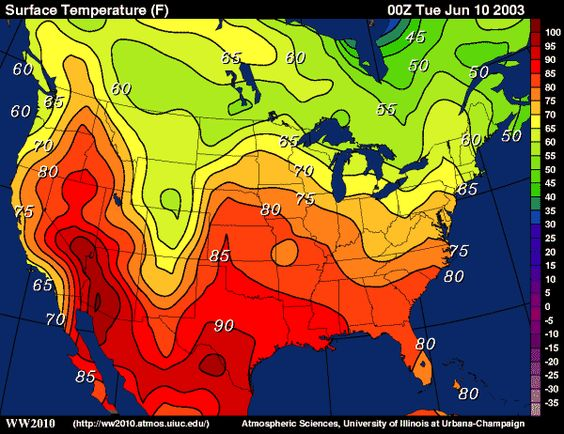
\includegraphics{isotherm.jpg}
\end{image}

Given a function $z=F(x,y)$, we can draw a ``topographical map'' of
$F$ by drawing \dfn{level curves} (or, contour lines). A level curve
at $z=c$ is a curve in the $(x,y)$-plane such that for all points
$(x,y)$ on the curve, $F(x,y) = c$. Below we see a surface with level
curves drawn beneath the surface:

\begin{image}
  %% Based on: 
  %% http://tex.stackexchange.com/questions/87674/how-to-coherently-combine-3d-and-contour-plots-with-pgfplots
\begin{tikzpicture}
\begin{axis}[
    domain=-2:2,
    domain y=0:2*pi,
]

    \newcommand\expr[2]{-exp(-#1^2) * sin(deg(#2))}

    \addplot3[%% Contour plot
        contour gnuplot={
            % cdata should not be affected by z filter:
            output point meta=rawz,
            number=10,
            labels=false,
        },
        samples=41,
        z filter/.code=\def\pgfmathresult{-1.6},
    ]
        {\expr{x}{y}};

        
    \addplot3[surf,samples=25] %% ACTUAL FUNCTION
        {\expr{x}{y}};

\end{axis}
\end{tikzpicture}
\end{image}

%% \begin{question} BADBAD Bart would like to add a question here
%%   Matching level curves to surfaces.
%% \end{question}


When drawing level curves, it is important that the $c$ values are
spaced equally apart as that gives the best insight to how quickly the
``elevation'' is changing. Examples will help one understand this
concept.

\begin{example}
  Let $F(x,y) = \sqrt{1-\frac{x^2}{9}-\frac{y^2}{4}}$. Find the level
  curves of $f$ for $c=0$, $0.2$, $0.4$, $0.6$, $0.8$ and $1$.
  \begin{explanation}
    Let's work somewhat generally. Each of our level curves will be of
    the form
    \begin{align*}
      c &= \sqrt{1-\frac{x^2}{9}-\frac{y^2}{4}}\\
        c^2 &= \answer[given]{1-\frac{x^2}{9}-\frac{y^2}{4}}.
    \end{align*}
    Now we just need to plot each of the following implicit functions:
    \begin{align*}
      0^2   &= 1-\frac{x^2}{9}-\frac{y^2}{4}, \\
      0.2^2 &= 1-\frac{x^2}{9}-\frac{y^2}{4}, \\
      0.4^2 &= 1-\frac{x^2}{9}-\frac{y^2}{4}, \\
      0.6^2 &= 1-\frac{x^2}{9}-\frac{y^2}{4}, \\
      0.8^2 &= 1-\frac{x^2}{9}-\frac{y^2}{4}, \\
        1^2 &= 1-\frac{x^2}{9}-\frac{y^2}{4}.   
    \end{align*}
    You can now plot these implicit functions with your favorite
    graphing device.
    \begin{onlineOnly}
      As a gesture of friendship, we have included a graph of these
      level curves:
      \[
      \graph[xmin=-5, xmax=5, ymin=-2.3, ymax=2.3]{0^2 = 1-\frac{x^2}{9}-\frac{y^2}{4}, 0.2^2 = 1-\frac{x^2}{9}-\frac{y^2}{4}, 0.4^2 = 1-\frac{x^2}{9}-\frac{y^2}{4},0.6^2 = 1-\frac{x^2}{9}-\frac{y^2}{4},0.8^2 = 1-\frac{x^2}{9}-\frac{y^2}{4},1^2 = 1-\frac{x^2}{9}-\frac{y^2}{4}}
      \]
    \end{onlineOnly}
    In the image below, the level curves are drawn on a graph of $F$
    in space.
    \begin{image}
      \begin{tikzpicture}
        \begin{axis}%
          [tick label style={font=\scriptsize},axis on top,
	    axis lines=center,
	    view={135}{25},
	    name=myplot,
	    %xtick=\empty,
	    %ytick=\empty,
	    %ztick=\empty,
	    ymin=-3.1,ymax=3.1,
	    xmin=-3.1,xmax=3.1,
	    zmin=-.1, zmax=2.1,
	    every axis x label/.style={at={(axis cs:\pgfkeysvalueof{/pgfplots/xmax},0,0)},xshift=-3pt,yshift=-3pt},
	    xlabel={\scriptsize $x$},
	    every axis y label/.style={at={(axis cs:0,\pgfkeysvalueof{/pgfplots/ymax},0)},xshift=5pt,yshift=-2pt},
	    ylabel={\scriptsize $y$},
	    every axis z label/.style={at={(axis cs:0,0,\pgfkeysvalueof{/pgfplots/zmax})},xshift=0pt,yshift=4pt},
	    zlabel={\scriptsize $z$},colormap/cool
	  ]
          \addplot3[domain=0:180,mesh,y domain=0:180,samples y=30,very thin,z buffer=sort,samples=30,] ({3*cos(x)*cos(y)},{2*sin(x)*cos(y)},{sin(y)});
          
          \addplot3 [very thick,penColor, smooth,domain=-40:170,samples=60,samples y=0] ({3*(cos(x))},{2*(sin(x))},0);

          \addplot3 [very thick,penColor, smooth,domain=-40:170,samples=60,samples y=0] ({2.93*(cos(x))},{1.96*(sin(x))},.2);
          
          \addplot3 [very thick,penColor, smooth,domain=-40:170,samples=60,samples y=0] ({2.75*(cos(x))},{1.83*(sin(x))},.4);
          
          \addplot3 [very thick,penColor, smooth,domain=-40:170,samples=60,samples y=0] ({2.4*(cos(x))},{1.6*(sin(x))},.6);
          
          \addplot3 [very thick,penColor, smooth,domain=-40:170,samples=60,samples y=0] ({1.8*(cos(x))},{1.2*(sin(x))},.8);
          
          %\filldraw [penColor] (axis cs: 0,0,1) circle (1pt);          
        \end{axis}
      \end{tikzpicture}
    \end{image}
    Note how the elevations are evenly spaced. Near the
    level curves of $c=0$ and $c=0.2$ we can see that $F$ indeed is
    growing quickly.
  \end{explanation}
\end{example}

If one example is good, two is better.

\begin{example}
  Let $F(x,y) = \frac{x+y}{x^2+y^2+1}$. Find the level curves for $z=c$.
  \begin{explanation}
    We begin by setting $F(x,y)=c$ for an arbitrary $c$ and seeing if
    algebraic manipulation of the equation reveals anything
    significant.
    \begin{align*}
      \frac{x+y}{x^2+y^2+1} &= c \\
      x+y &= \answer[given]{c(x^2+y^2+1)}.
    \end{align*}
    You may recognize this as a circle; regardless, plotting
    \[
    x+y = c(x^2+y^2+1).
    \]
    for $c=0,\pm 0.2$, $\pm 0.4$, and $\pm 0.6$ will reveal the shape of the
    surface defined by $F$.
    \begin{onlineOnly}
      As a gesture of friendship, we have included a graph of these
      level curves:
      \[
      \graph[xmin=-15, xmax=15, ymin=-7, ymax=7]{x+y = 0.6(x^2+y^2+1),x+y = 0.4(x^2+y^2+1), x+y = 0.2(x^2+y^2+1),x+y = 0,x+y = -0.2(x^2+y^2+1),x+y = -0.4(x^2+y^2+1),x+y = -0.6(x^2+y^2+1)}
      \]
    \end{onlineOnly}
    \begin{image}
      \begin{tikzpicture}
        \begin{axis}%
          [tick label style={font=\scriptsize},axis on top,
	    axis lines=center,
	    view={30}{30},
	    name=myplot,
            %width=5in,
	    %xtick=\empty,
	    %ytick={5},
	    %ztick={.7,-.7},
	    ymin=-6.6,ymax=6.6,
	    xmin=-6.6,xmax=6.6,
	    zmin=-.8, zmax=.8,
	    every axis x label/.style={at={(axis cs:\pgfkeysvalueof{/pgfplots/xmax},0,0)},xshift=5pt,yshift=0pt},
	    xlabel={\scriptsize $x$},
	    every axis y label/.style={at={(axis cs:0,\pgfkeysvalueof{/pgfplots/ymax},0)},xshift=4pt,yshift=2pt},
	    ylabel={\scriptsize $y$},
	    every axis z label/.style={at={(axis cs:0,0,\pgfkeysvalueof{/pgfplots/zmax})},xshift=0pt,yshift=4pt},
	    zlabel={\scriptsize $z$},
            colormap/cool
	  ]
          \addplot3[domain=-6.5:6.5,y domain=-6.5:6.5,mesh,samples y=30,very thin,z buffer=sort,
            samples=30,] {(x+y)/(x^2+y^2+1)};
          \addplot3 [very thick,penColor, smooth,domain=0:360,samples=60,samples y=0] ({-0.833333 + 0.62361*cos(x)},{-0.833333 + 0.62361*sin(x)},-.6);
          \addplot3 [very thick,penColor, smooth,domain=0:360,] ({-1.25 + 1.45774*cos(x)}, {-1.25 + 1.45774*sin(x)},-.4);
          \addplot3 [very thick,penColor, smooth,domain=0:360,] ({-2.5 + 3.39116*cos(x)},{-2.5 + 3.39116*sin(x)},-.2);
          \addplot3 [very thick,penColor,domain=-5:5] (x,-x,0);
          \addplot3 [very thick,penColor, smooth,domain=0:360,] ({2.5 + 3.39116*cos(x)}, {2.5 + 3.39116*sin(x)},.2);
          \addplot3 [very thick,penColor, smooth,domain=0:360,] ({1.25 + 1.45774*cos(x)},{1.25 + 1.45774*sin(x)},.4);
          \addplot3 [very thick,penColor, smooth,domain=0:360,] ({0.833333 + 0.62361*cos(x)},{0.833333 + 0.62361*sin(x)},.6);
          %\filldraw [penColor] (axis cs: 0,0,1) circle (1pt);
        \end{axis}
      \end{tikzpicture}
    \end{image}
    Seeing the level curves helps us understand the graph. For
    instance, the graph does not make it clear that one can ``walk''
    along the line $y=-x$ without elevation change, though the level
    curve does.
  \end{explanation}
\end{example}


\subsection{Level surfaces}


It is very difficult to produce a meaningful graph of a function of
three variables.
\begin{itemize}
  \item A function of \textbf{one} variable is a \textbf{curve} drawn
    in \textbf{two} dimensions.
  \item A function of \textbf{two} variables is a \textbf{surface}
    drawn in \textbf{three} dimensions.
  \item A function of \textbf{three} variables is a
    \textbf{hypersurface} drawn in \textbf{four} dimensions.
\end{itemize}

There are a few techniques one can employ to try to ``picture'' a
graph of three variables. One is an analogue of level curves:
\dfn{level surfaces}. Given $w=f(x,y,z)$, the level surface at $w=c$
is the surface in space formed by all points $(x,y,z)$ where
$f(x,y,z)=c$. Time for an example.


\begin{example}
  If a point source $S$ is radiating energy, the intensity $I$ at a
  given point $P$ in space is inversely proportional to the square of
  the distance between $S$ and $P$. That is, when $S=(0,0,0)$,
  \begin{align*}
  I(x,y,z) &= \frac{\text{some constant}}{\text{distance squared}}\\
  &=\frac{k}{x^2+y^2+z^2}
  \end{align*}
  for some constant $k$.  Let $k=1$; find the level surfaces of $I$.
  \begin{explanation}
    We can (mostly) answer this question using ``common sense.'' If
    energy (say, in the form of light) is emanating from the origin,
    its intensity will be the same all a points equidistant from the
    origin. That is, at any point on the surface of a sphere centered
    at the origin, the intensity should be the same. Therefore, the
    level surfaces are spheres.
    
    We now confirm this ``common sense'' mathematically. The level
    surface at $I=c$ is defined by
    \[
    c = \frac{1}{x^2+y^2+z^2}.
    \]
    Algebra reveals
    \[
    \answer[given]{x^2+y^2+z^2} = \frac{1}{c}.
    \]
    Given an intensity $c$, the level surface $I=c$ is a sphere of
    radius $1/\sqrt{c}$, centered at the origin. Every point on each
    sphere experiences the same intensity of the radiating energy.
    \begin{onlineOnly}
      For your viewing pleasure, we present the level surface of this
      curve graphed by \sage. Here $c$ is the intensity. 
\begin{sageCell}
c=16;
f(x,y,z) = x^2 + y^2 + z^2
implicit_plot3d(f==1/c,(x,-1,1), (y,-1,1), (z,-1,1))
\end{sageCell}
\begin{question}
  If the distance is doubled, is the intensity halved?
  \begin{multipleChoice}
    \choice{yes}
    \choice[correct]{no}
  \end{multipleChoice}
  \begin{feedback}
    Experiment with how the level surface changes when the intensity
    is halved. We can see that that the closer one is to the source,
    the more rapidly the intensity changes.
  \end{feedback}
\end{question}
    \end{onlineOnly}
  \end{explanation}
\end{example}
%% \begin{tikzpicture}             
%%   \begin{axis}
%% 	\addplot3[contour gnuplot,samples=100]
%% 		{exp(0-x^2-y^2)};
%% 	\end{axis}
%% \end{tikzpicture}
\end{document}
